\section{FORESEE}

\subsection{Dataset}

In this experiment, we use datasets from the PubDAS \cite{spica2023pubdas} collection. PubDAS is described as "A PUBlic Distributed Acoustic Sensing Datasets Repository for Geosciences" and contains \acrshort{das} data from numerous locations worldwide. We will specifically be dealing with the FORESEE \cite{zhu2019penn} dataset, a \acrshort{das} dataset from an area around Pennsylvania in the Valley and Ridge Appalachians region as seen in figure \ref{fig:foresee}. \\

\begin{figure}[!h]
    \centering
    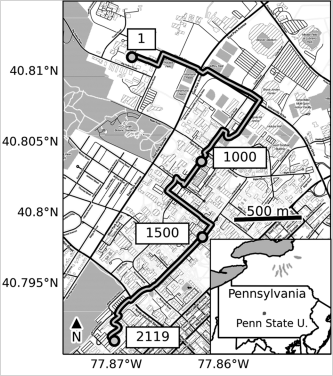
\includegraphics[width=0.5\linewidth]{figures/foresee.png}
    \caption{Map of the FORESEE Array. Photo is taken the PubDAS paper \cite{spica2023pubdas}}
    \label{fig:foresee}
\end{figure}

\subsubsection{Data Preprocessing}
\label{exp:fordata}

\begin{table}[!h]
    \centering
    \small
    \begin{tabular}{@{}p{0.3\textwidth}p{0.3\textwidth}p{0.3\textwidth}@{}}
        \toprule
        \textbf{Parameter} & \multicolumn{2}{l}{\textbf{Value}} \\
        \midrule
        Experiment & \multicolumn{2}{l}{Foresee}  \\
        Interrogator Unit (IU) & \multicolumn{2}{l}{Silixa iDAS-v2}  \\
        Gauge length & \multicolumn{2}{l}{\qty{10}{\si{\meter}}} \\
        Cable length & \multicolumn{2}{l}{\qty{23300}{\si{\meter}}} \\
        Channel spacing & \multicolumn{2}{l}{\qty{2}{\si{\meter}}} \\
        \midrule
        & \textbf{Original Data} & \textbf{After Preprocessing} \\
        \cmidrule(lr){2-3}
        Format & TDMS & HDF5 \\
        Sample rate & \qty{500}{\si{\hertz}} & \qty{125}{\si{\hertz}} \\
        File duration & \qty{10}{\si{\minute}} & \qty{5}{\si{\second}} \\
        Data shape & 300000 \(\times\) 2137 & 625 \(\times\) 2137 \\
        Datatype & Float32 & Float32 \\
        File size & \qty{2.5644}{\si{\giga\byte}} & \qty{4.98}{\si{\mega\byte}} \\
        \midrule
        \textbf{Dataset Information} & \multicolumn{2}{l}{} \\
        Train dataset size & \multicolumn{2}{l}{\qty{25690}{files}} \\
        Train dataset span & \multicolumn{2}{l}{02 Mar 2020 08:10:15 to 03 Mar 2020 20:40:10} \\
        Anomalous dataset size & \multicolumn{2}{l}{\qty{600}{files}} \\
        Anomalous dataset span & \multicolumn{2}{l}{15 Apr 2019 03:17:35 to 15 Apr 2019 04:07:30} \\
        \bottomrule
    \end{tabular}
    \caption{FORESEE Experiment Data Summary}
    \label{tab:foresee_experiment_data}
\end{table}

Preprocessing of the dataset has already been performed, as detailed in Appendix \ref{app:pubdas}. The files have been converted to the \acrshort{hdf5} format and the data resampled. Due to memory constraints of most consumer-grade \acrshort{gpu}s, which typically have around 8-32 GB of VRAM, the number of 10-minute data batches that can be processed simultaneously is limited. This constraint is worsened by the need to further store the model's weights, biases, and computed losses in VRAM.
To address these limitations and enhance the system's responsiveness, we chose to split the files into 5-second segments instead of the original 10-minute recordings. This approach offers two major advantages:

\begin{itemize}
    \item It allows for training across various GPU architectures, accommodating different memory capacities.
    \item It enables more frequent updates in online anomaly detection, potentially identifying anomalous events every 5 seconds, dramatically improving the system's real-time response capability.
\end{itemize}


The file-splitting process was implemented in parallel using Julia, resulting in a collection of nearly 26,000 files for our training dataset.This preprocessing strategy mitigates hardware constraints and aligns with the requirements of real-time or near-real-time anomaly detection systems, where rapid identification of anomalies is crucial. A crucial aspect of our approach concerns the composition of the training dataset:

\begin{enumerate}
    \item \textit{Precense of anomalies}: The training dataset \textit{may} contain some anomalous data. This deliberate decision reflects real-world scenarios where completely ``clean'' data is rare.
    \item \textit{Time period selection}: We attempt to mitigate this by selecting a time period with minimal documented extreme weather events, earthquakes, or other known anomalous occurrences. This approach aims to minimize, but not entirely eliminate, the presence of anomalies in the training data.
    \item \textit{Model robustness}: By including potential anomalies in the training set, we aim to examine whether our models are sufficiently robust to withstand and learn from data that may contain a small proportion of anomalous samples.
    \item \textit{Unsupervised learning}: Although labeled anomalies technically place our approach in the realms of self-supervised learning, our goal is to develop models that can effectively identify anomalies despite this challenge. Possibly remove?
\end{enumerate}

It's important to note that while data quality and quantity are paramount in deep learning, we've consciously decided to balance preprocessing effort with practical considerations. Our approach aims to reduce the time and resources spent on extensive preprocessing, reflecting real-world constraints where perfect data cleaning may not always be feasible or economically viable. Information about the data can be found in table \ref{tab:foresee_experiment_data}. \\

Finally, we select a test dataset for labeling anomalies based on the findings of Zhu et al. (2023) \cite{zhu2023seismic}, who identified 18 thunder-induced seismic events between 03:20 and 03:50 on the day in question. We manually label each file as either anomalous or non-anomalous. This labeled dataset enables us to calculate confusion matrices and other relevant metrics to evaluate the accuracy of our autoencoders. Our approach can thus be described as unsupervised learning with supervised evaluation.

%TODO: Inference data from 15042019!


\subsection{Experiment \rnum{1}: Model training and Reconstruction}


\begin{table}[!h]
\centering
\small
\rowcolors{2}{gray!15}{white} % Start with the second row, alternate between light gray and white
\begin{tabular}{@{}lllll@{}}
\toprule
\rowcolor{gray!30} % Darker gray for the header row
\textbf{Parameter} & \textbf{AE} & \textbf{$\beta$-VAE} & \textbf{CAE} & \textbf{$\beta$-CVAE} \\
\midrule
Files & 25600 & 25600 & 25600 & 25600 \\
Input Shape & [BS, 625 × 2137] & [BS, 625 × 2137] & [BS, 1, 625, 2137] & [BS, 1, 625, 2137] \\
Batch Size & 256 & 256 & 32 & 32 \\
Validation Split & 0.2 & 0.2 & 0.2 & 0.2 \\
Epochs & 200 & 200 & 200 & 200 \\
Seed & 1337 & 1337 & 1337 & 1337 \\
Loss Function & \acrshort{mse} & \acrshort{elbo} & \acrshort{mse} & \acrshort{elbo} \\
Optimizer & ADAM & ADAM & ADAM & ADAM \\
Learning Rate & 0.001 & 0.001 & 0.002 & 0.001 \\
LR Scheduler & ReduceOnPlateau & ReduceOnPlateau & ReduceOnPlateau & ReduceOnPlateau \\
LR Scheduler Patience & 5 & 5 & 5 & 5 \\
LR Scheduler Factor & 0.5 & 0.5 & 0.5 & 0.5 \\
Early Stopping Patience & 10 & 10 & 10 & 10 \\
Early Stopping Min $\Delta$ & 0.0001 & 0.0001 & 0.0001 & 0.0001 \\
\bottomrule
\end{tabular}
\caption{Hyperparameters for all models}
\label{tab:hyperparameters}
\end{table}




In this first experiment, we train four different autoencoders and examine their reconstruction capabilities, focusing on reconstruction loss, median- and overall training time. These four models are a dense regular autoencoder (AE \ref{app:a-ae}), a variational autoencoder ($\beta$-VAE \ref{app:a-vae}), and convolutional variants of both (CAE \ref{app:a-cae} and $\beta$-CVAE \ref{app:a-cvae}). \\ 

As shown in table \ref{tab:hyperparameters}, the model sizes differ quite drastically, which aligns with our expectations based on their architectures. Convolutional layers typically require fewer parameters than linear layers, resulting in convolutional autoencoders needing less memory. However, we need to decrease the batch size for convolutional models since each convolutional layer operates on higher-dimensional data, increasing GPU memory usage during training. Additionally, the \acrshort{vae} models require extra parameters since the latent layer is represented by both $\mu$ and $\sigma$ layers, slightly increasing their size compared to their non-variational counterparts. Detailed descriptions of all the models and their layer structures can be found in Appendix \ref{app:archs}. \\

We selected these hyperparameters based on a combination of literature review and preliminary experiments. The relatively large batch sizes (256 for dense models, 32 for convolutional) allow for stable gradient updates, while the learning rate of 0.001 is a common starting point for the \acrshort{adam} optimizer \cite{kingma2017adam}. To optimize the training process, we introduce a learning rate scheduler that reduces the learning rate by half if the validation loss does not decrease over 5 epochs. Combined with an early-stop mechanism described in the section, we can attempt escaping local minima and stop unnecessary training whenever the validation loss does not decrease by at least $\Delta$ (0.0001) by 10 consecutive epochs. \\ 

To evaluate and compare the reconstruction capabilities of these models, we will primarily use the \acrshort{mse} for the AE and CAE, and  \acrshort{elbo} loss with \acrshort{mse} for $\mathcal{L}_{rec}$ for the $\beta$-VAE and $\beta$-CVAE, as described in section \ref{back:elbo}. We will also visually inspect reconstructed samples to assess the models' performance qualitatively.



\subsection{Experiment \rnum{2}: Anomaly Detection}
Without a real-time feed of \acrshort{das} data, we use a labeled dataset to evaluate the different models' capabilities for anomaly detection, as described in section \ref{exp:fordata}. From this, we compute a confusion matrix and evaluate the models based on the following metrics:

\begin{itemize}
    \item Precision: The percentage of correct anomalies out of all predicted anomalies.
    \begin{equation}
        Precision = \frac{TP}{TP + FP}
    \end{equation}

    \item True Positive Rate (TPR), also known as recall: The percentage of correctly identified anomalies out of all actual anomalies.
    \begin{equation}
        TPR = Recall = \frac{TP}{TP + FN}
    \end{equation}

    \item F1-score: Used to evaluate the balance between precision and recall; the higher the score, the better. 
    \begin{equation}
        F1_{score} = 2 \times \frac{Precision \cdot Recall}{Precision + Recall}
    \end{equation}

    \item False Positive Rate (FPR): The percentage of normal windows incorrectly identified as anomalous. FPR is highly relevant for \acrshort{das} and other signal systems, where false alarms may be costly. A low FPR indicates that normal data is not misclassified as anomalous; thus, the lower the score, the better.
    \begin{equation}
        FPR = \frac{FP}{FP + TN}
    \end{equation}
\end{itemize}

In addition to these metrics, we will also use the \acrfull{pr} curve and the \acrshort{pr} \acrfull{auc}. The PR curve is particularly useful for imbalanced datasets, which are common in anomaly detection tasks.

As seen in Figure~\ref{fig:dataflow}, we ultimately want to find our models' optimal threshold score $\epsilon^*$. To find $\epsilon^*$, we analyze how precision, recall, and F1-score change across different threshold values, identifying the best anomaly score threshold. This operation is highlighted in \ref{alg:thresh}.  

\begin{algorithm}[!h]
\caption{Optimal Threshold Selection Algorithm}
\label{alg:thresh}
\begin{algorithmic}[1]
\Require Model $\mathcal{M}$, Dataset $\mathcal{Y} = \{y_1, \ldots, y_N\}$, Anomaly Indices $\mathcal{I} = \{i : y_i \text{ is anomalous}\}$
\Ensure Optimal Threshold $\epsilon^*$
\State $\mathbf{e} \gets \mathcal{L}_{\text{MSE}}(\mathcal{Y}, \mathcal{M}(\mathcal{Y}))$ \Comment{MSE reconstruction errors}
\State $\mathbf{a} \gets \mathbf{0}_N$ \Comment{Initialize true anomaly bitvector}
\For{$i \in \mathcal{I}$}
    \State $a_i \gets 1$
\EndFor
\State $\mathbf{p}, \mathbf{r}, \boldsymbol{\theta} \gets \text{PRC}(\mathbf{a}, \mathbf{e})$ \Comment{PR-Curve}
\State $\mathbf{f} \gets 2 \cdot \frac{\mathbf{p} \odot \mathbf{r}}{\mathbf{p} + \mathbf{r}}$ \Comment{Element-wise operations}
\State $\epsilon^* \gets \theta_{\argmax(\mathbf{f})}$
\State \Return $\epsilon^*$
\end{algorithmic}
\end{algorithm}

\subsection{Experiment Setup}

All the models were trained and tested on \gls{idun} computers made for \acrshort{hpc}. Details of the machines used can be found in the table below. \\


\begin{table}[!htbp]
\centering
\caption{Specifications for Model Training and Testing Environment}
\label{tab:system-specs}
\begin{tabular}{@{}llr@{}}
\toprule
\textbf{Component} & \textbf{Description} & \textbf{Quantity} \\
\midrule
Operating System & Ubuntu Linux 22.04 LTS & 1 machine \\
GPU Model & NVIDIA H100 PCIe & 4 units \\
GPU Memory & HBM3 & 80 GB per GPU \\
CUDA Cores & & 14,592 per GPU \\
Tensor Cores & & 576 per GPU \\
GPU Clock Speed & Boost Clock & 1.67 GHz \\
GPU TDP & & 350 W \\
FP16 & & 204.9 TFLOPS \\
FP32 & & 51.22 TFLOPS \\
\midrule
\multicolumn{3}{@{}l@{}}{\textit{Note:} 1 \acrshort{gpu} dedicated for testing, 4 for training.} \\
\bottomrule
\end{tabular}
\end{table}